\documentclass{beamer}
\mode<presentation>
\usetheme{CambridgeUS}
\usepackage[russian]{babel}
\usepackage[utf8]{inputenc}
\usepackage[T2A]{fontenc}
\usepackage{sansmathaccent}

\usepackage{verbatim}
\usepackage{alltt}

\pdfmapfile{+sansmathaccent.map}
\title[Software Design]{UML - унифицированный язык моделирования}
\author{Наумов Д.А., доц. каф. КТ}
\date[16.09.2019] {Основы программной инженерии, 2019}

\begin{document}

%ТИТУЛЬНЫЙ СЛАЙД
\begin{frame}
  \titlepage
\end{frame}
  
%СОДЕРЖАНИЕ ЛЕКЦИИ
\begin{frame}
  \frametitle{Содержание лекции}
  \tableofcontents  
\end{frame}
  
\section{Визуальное моделирование и его средства}
%Диаграммы вариантов использования
%Диаграммы классов
%Рекомендации по изображению UML диаграмм

\begin{frame}[t]{Визуальное моделирование и его средства}
\begin{figure}[h]
\centering
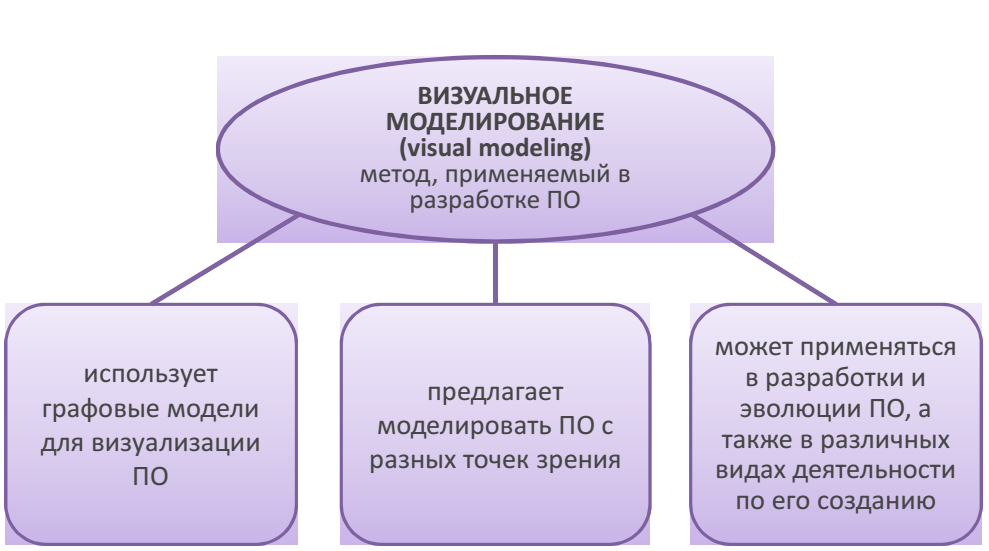
\includegraphics[scale=0.45]{images/lec03-pic01.png}
\end{figure}
\end{frame} 

\begin{frame}[t]{Язык UML}
\begin{block}{Унифицированный язык моделирования (UML)}
язык графического описания программных сущностей в виде диаграмм.
\end{block}
\begin{itemize}
\item диаграммы предметной области;
\item диаграммы предполагаемого дизайна;
\item диаграммы завершенной реализации;
\end{itemize}
Три уровня:
\begin{itemize}
\item концептуальный уровень;
\item уровень спецификации;
\item уровень реализации.
\end{itemize}
\end{frame}

\begin{frame}[t]{Визуальное моделирование и его средства}
Визуальное моделирование применяется на практике с помощью методов, языков и соответствующих программных инструментов.
\begin{figure}[h]
\centering
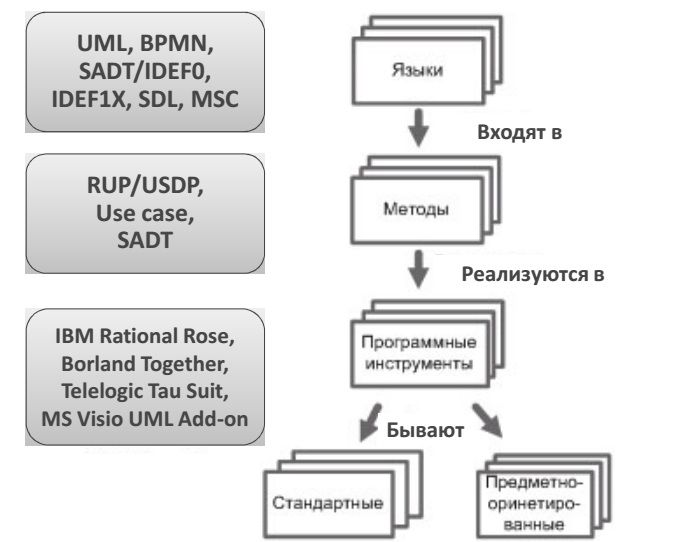
\includegraphics[scale=0.45]{images/lec03-pic02.png}
\end{figure}
\end{frame} 

\section{Понятие и применение UML}

\begin{frame}[t]{Язык UML}
Три вида диаграмм UML:
\begin{itemize}
\item статические - описывают неизменную логическую структуру программы, а именно элементы - классы, объекты, структуры данных - и отношения между ними;
\item динамические - показано, как программные сущности изменяются во время выполнения: поток выполнения или изменение состояния сущностей;
\item физические - изображается неизменная физическая структура системы: исходные файлы, библиотеки, двоичные файлы, файлы данных и прочее, а также связи между ними.
\end{itemize}
\end{frame}

\begin{frame}[t]{Понятие и применение UML}
\begin{figure}[h]
\centering
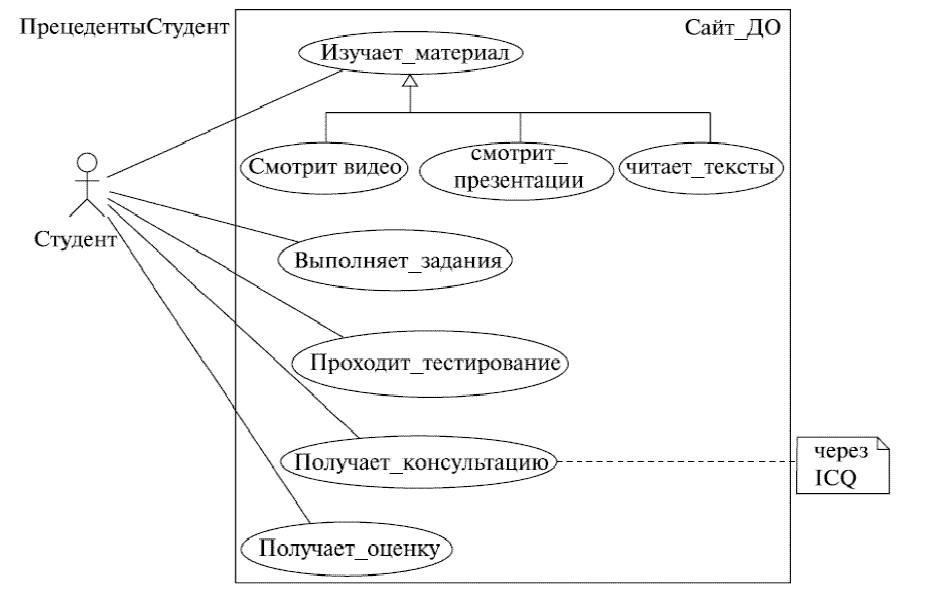
\includegraphics[scale=0.45]{images/lec03-pic03.png}
\end{figure}
\end{frame} 

\begin{frame}[t]{Понятие и применение UML}
\begin{figure}[h]
\centering
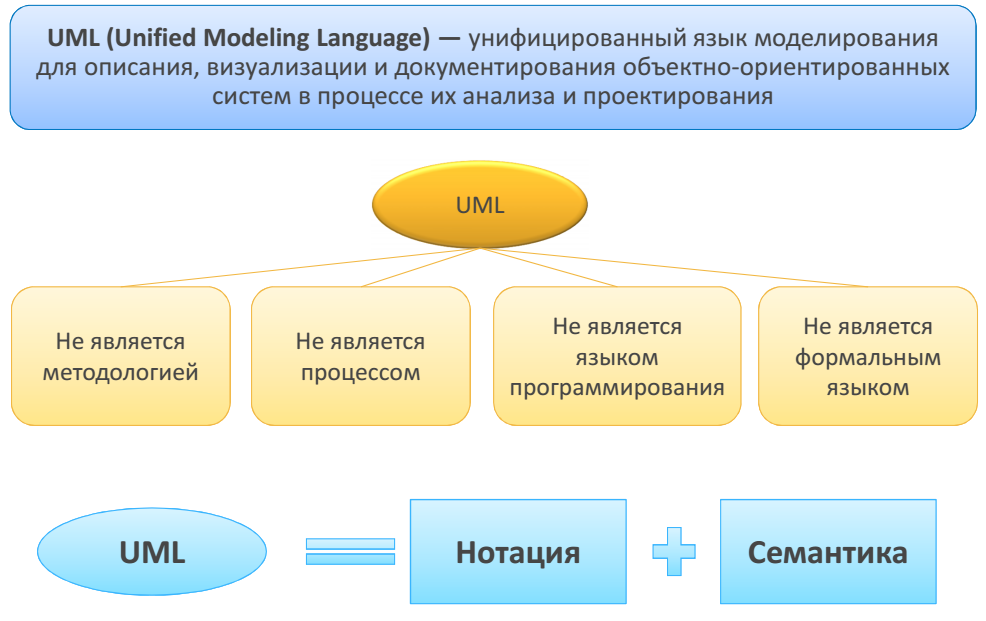
\includegraphics[scale=0.45]{images/lec03-pic04.png}
\end{figure}
\end{frame}

\begin{frame}[t]{Назначение UML}
\begin{figure}[h]
\centering
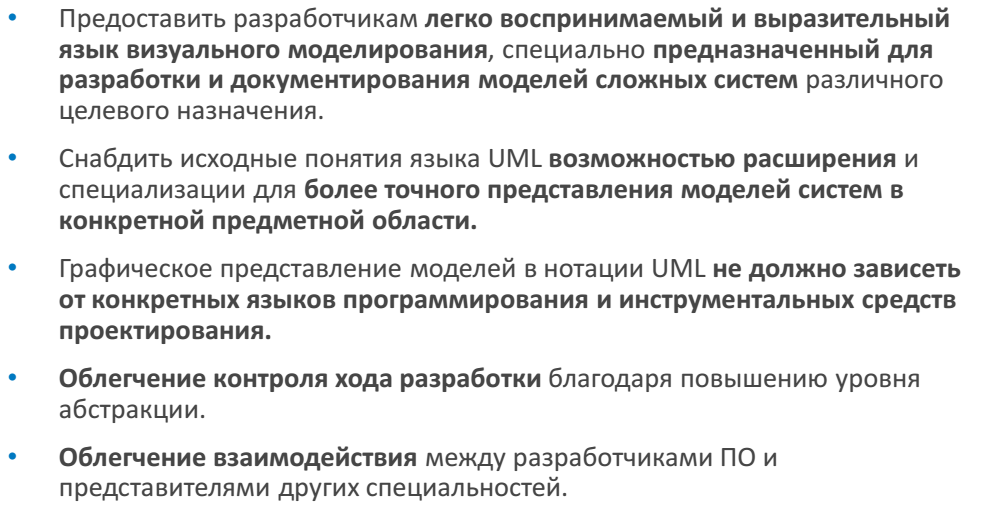
\includegraphics[scale=0.5]{images/lec03-pic05.png}
\end{figure}
\end{frame}

\section{Виды диаграмм UML}
\subsection{Диаграмма вариантов использования}

\begin{frame}[t]{Виды диаграмм UML}
\begin{figure}[h]
\centering
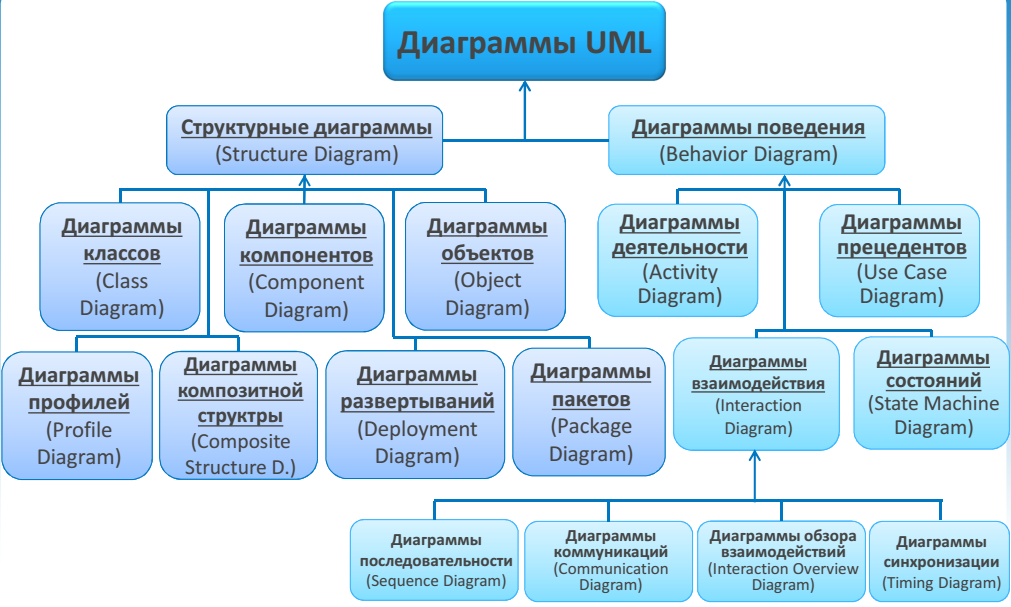
\includegraphics[scale=0.45]{images/lec03-pic06.png}
\end{figure}
\end{frame}

\begin{frame}[t]{Диаграмма вариантов использования}
\begin{figure}[h]
\centering
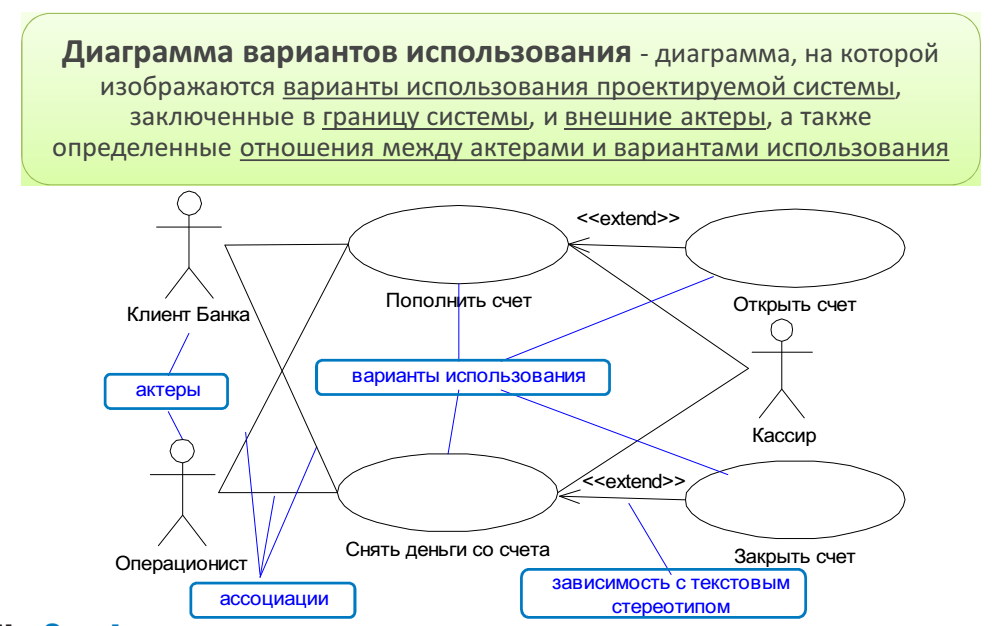
\includegraphics[scale=0.45]{images/lec03-pic07.png}
\end{figure}
\end{frame}

\begin{frame}[t]{Диаграмма вариантов использования}
\begin{figure}[h]
\centering
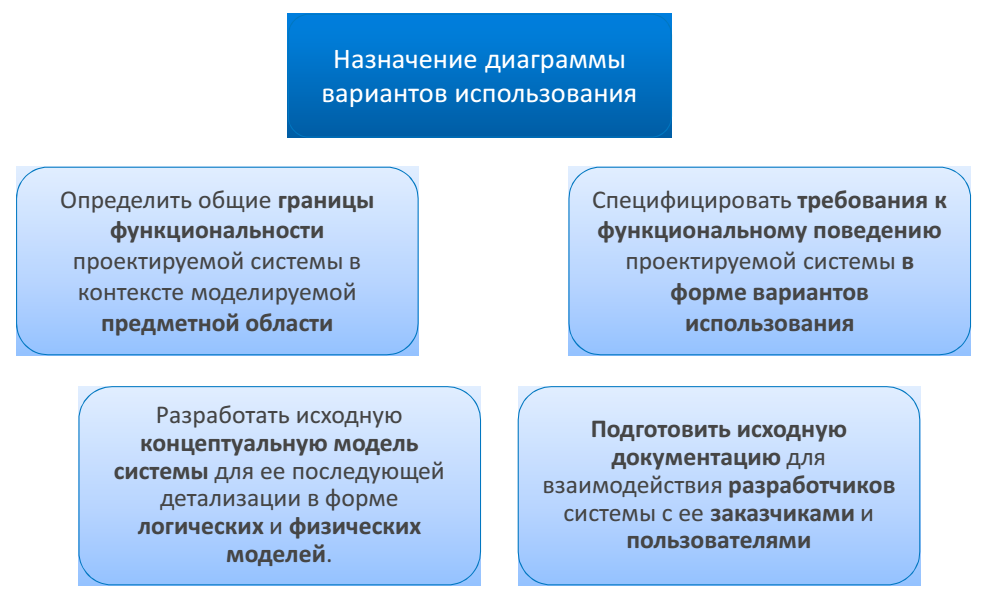
\includegraphics[scale=0.45]{images/lec03-pic08.png}
\end{figure}
\end{frame}

\begin{frame}[t]{Диаграмма вариантов использования}
\begin{figure}[h]
\centering
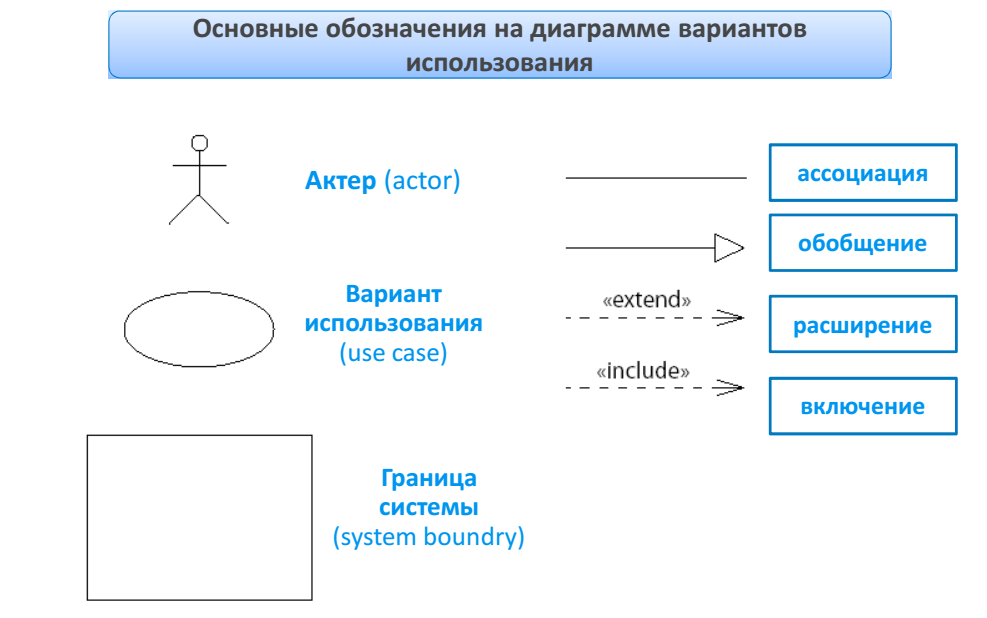
\includegraphics[scale=0.45]{images/lec03-pic09.png}
\end{figure}
\end{frame}

\begin{frame}[t]{Диаграмма вариантов использования}
\begin{figure}[h]
\centering
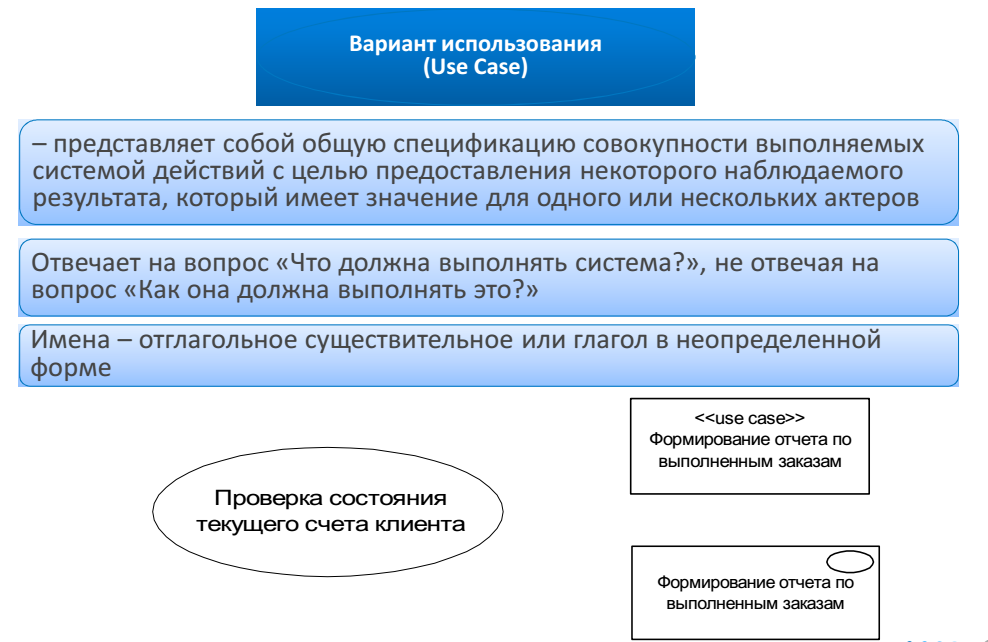
\includegraphics[scale=0.45]{images/lec03-pic10.png}
\end{figure}
\end{frame}

\begin{frame}[t]{Диаграмма вариантов использования}
\begin{figure}[h]
\centering
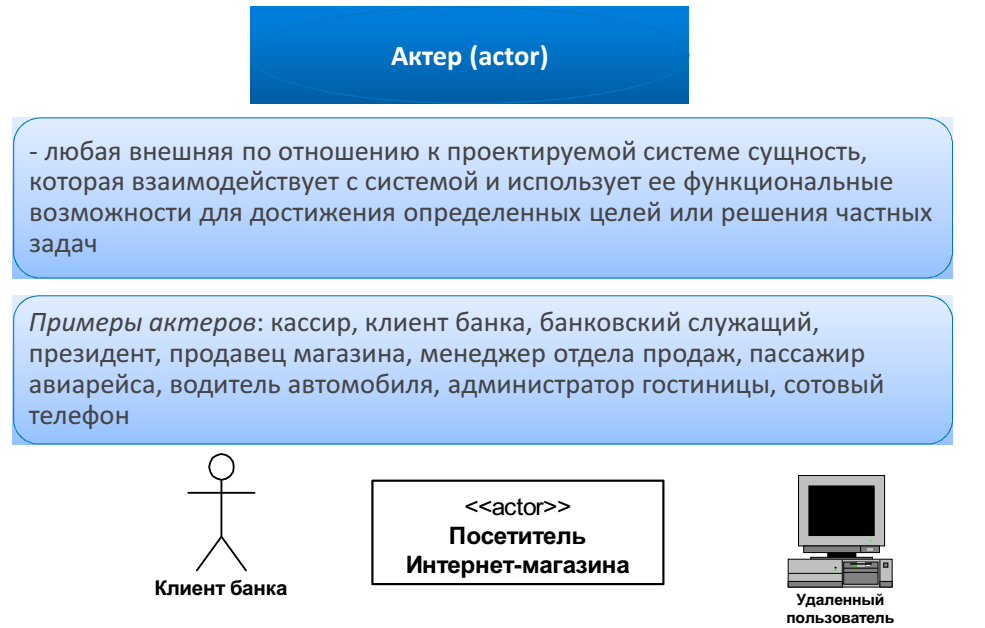
\includegraphics[scale=0.45]{images/lec03-pic11.png}
\end{figure}
\end{frame}

\begin{frame}[t]{Диаграмма вариантов использования}
\begin{figure}[h]
\centering
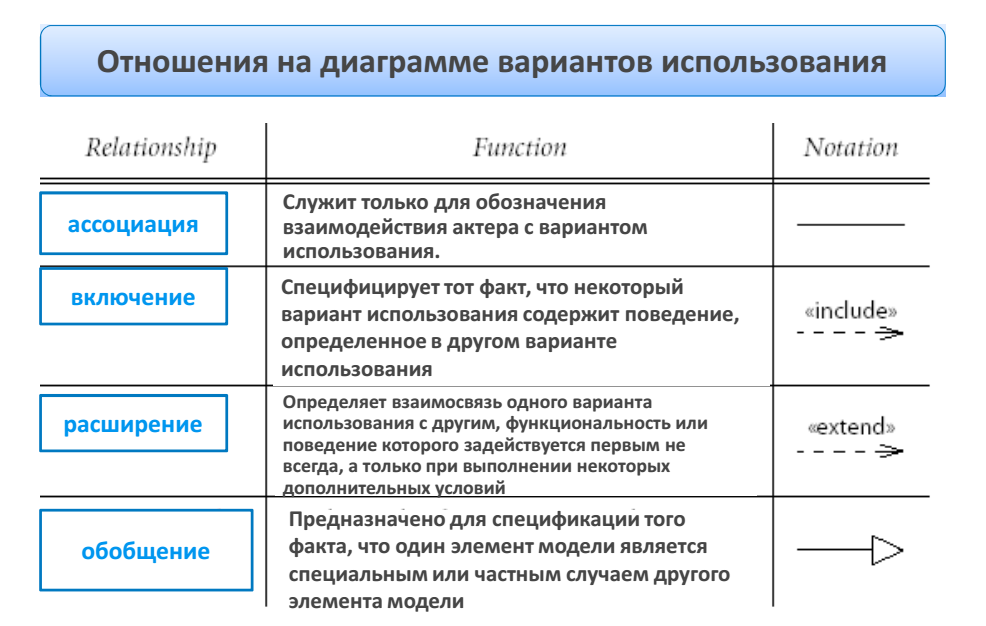
\includegraphics[scale=0.45]{images/lec03-pic12.png}
\end{figure}
\end{frame}

\begin{frame}[t]{Диаграмма вариантов использования}
\begin{figure}[h]
\centering
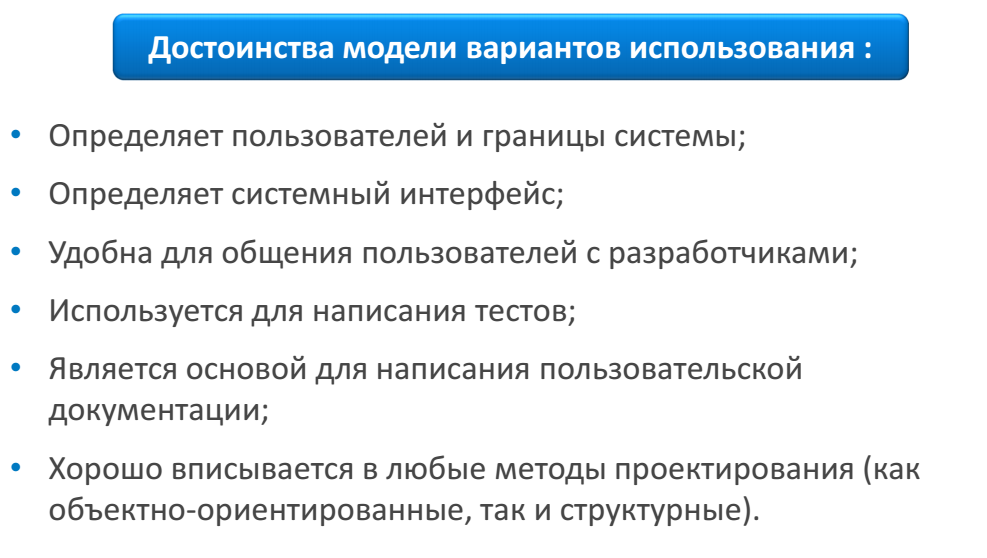
\includegraphics[scale=0.45]{images/lec03-pic13.png}
\end{figure}
\end{frame}

\subsection{Диаграмма классов}

\begin{frame}[t]{Диаграмма классов}
\begin{figure}[h]
\centering
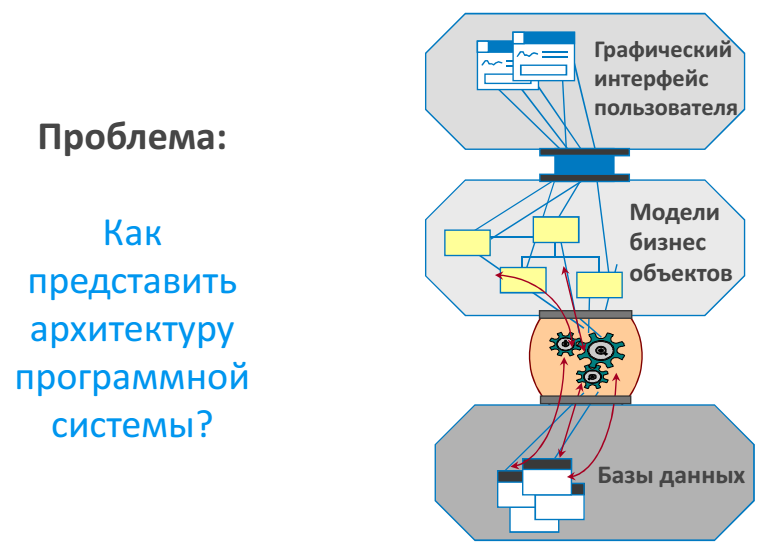
\includegraphics[scale=0.45]{images/lec03-pic14.png}
\end{figure}
\end{frame}

\begin{frame}[t]{Диаграмма классов}
\begin{figure}[h]
\centering
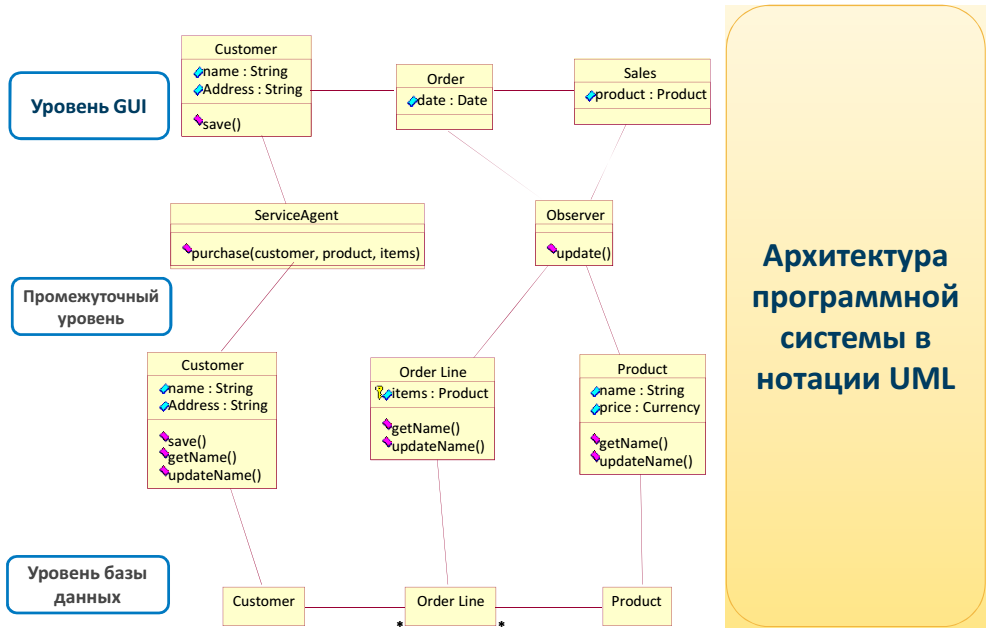
\includegraphics[scale=0.45]{images/lec03-pic15.png}
\end{figure}
\end{frame}

\begin{frame}[t]{Диаграмма классов}
\begin{figure}[h]
\centering
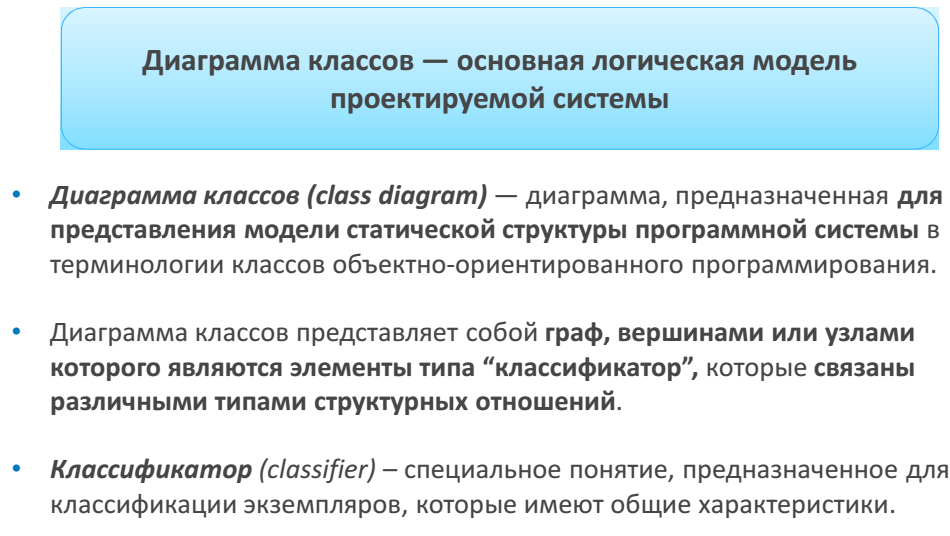
\includegraphics[scale=0.45]{images/lec03-pic16.png}
\end{figure}
\end{frame}

\begin{frame}[t]{Диаграмма классов}
\begin{figure}[h]
\centering
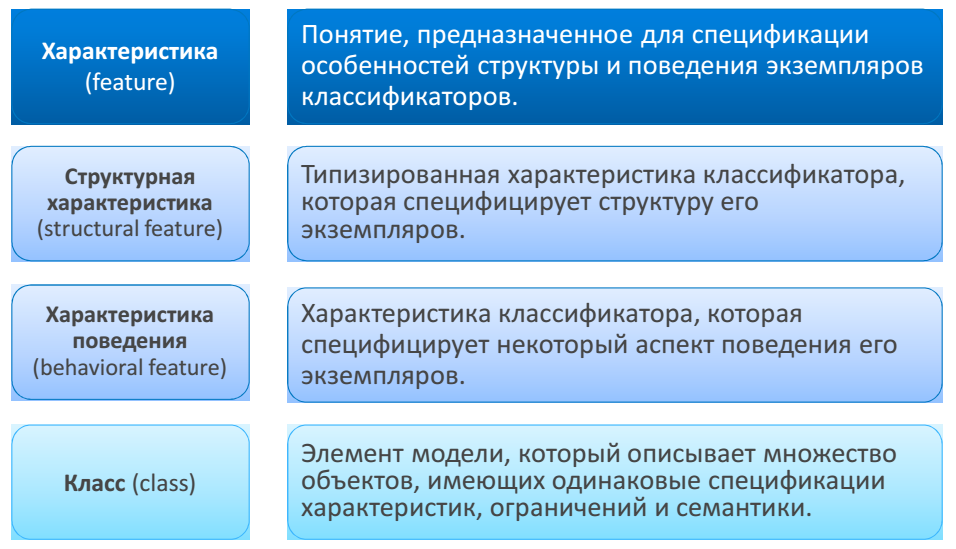
\includegraphics[scale=0.45]{images/lec03-pic17.png}
\end{figure}
\end{frame}

\begin{frame}[t]{Диаграмма классов}
\begin{figure}[h]
\centering
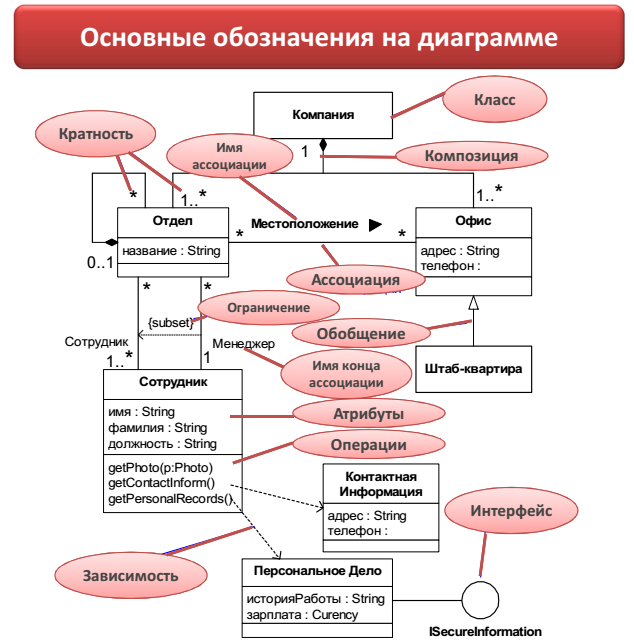
\includegraphics[scale=0.45]{images/lec03-pic18.png}
\end{figure}
\end{frame}

\begin{frame}[t]{Диаграмма классов}
\begin{figure}[h]
\centering
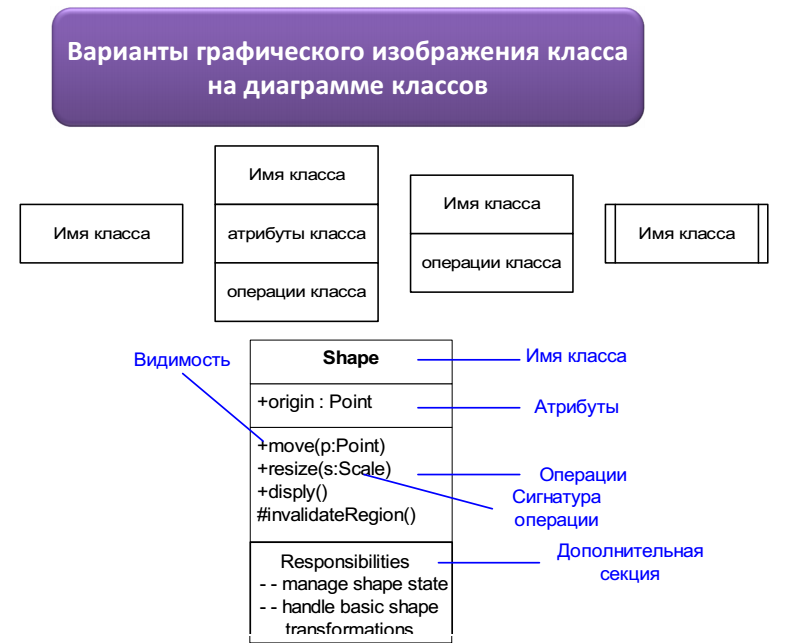
\includegraphics[scale=0.45]{images/lec03-pic19.png}
\end{figure}
\end{frame}

\begin{frame}[t]{Диаграмма классов}
\begin{figure}[h]
\centering
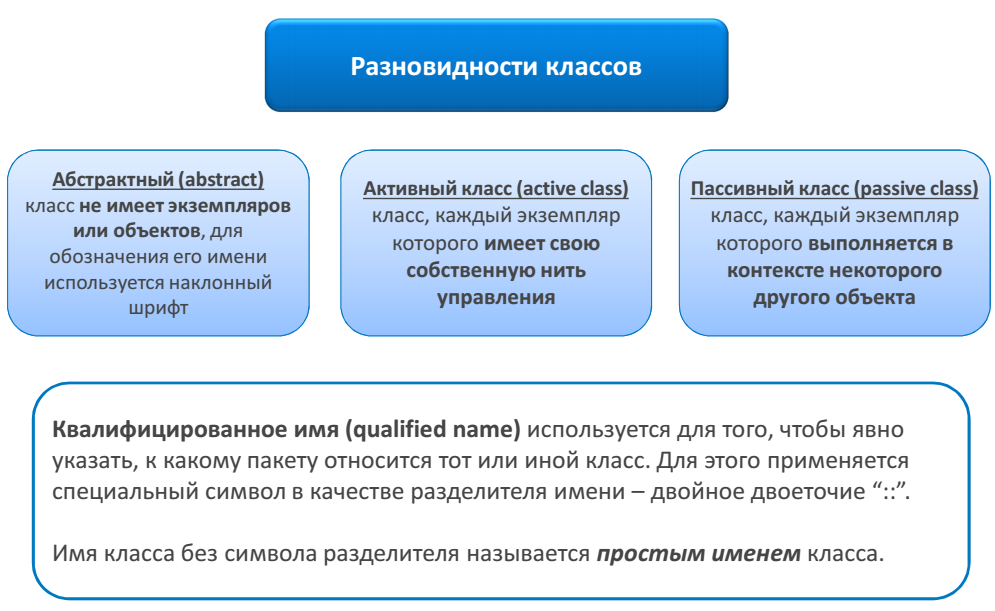
\includegraphics[scale=0.45]{images/lec03-pic20.png}
\end{figure}
\end{frame}

\begin{frame}[t]{Диаграмма классов}
\begin{figure}[h]
\centering
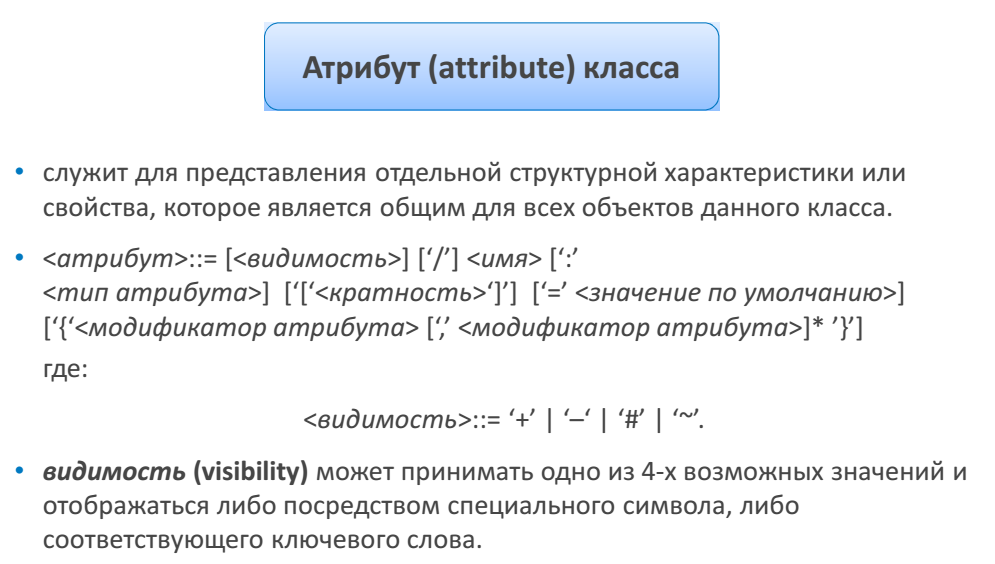
\includegraphics[scale=0.45]{images/lec03-pic21.png}
\end{figure}
\end{frame}

\begin{frame}[t]{Диаграмма классов}
\begin{figure}[h]
\centering
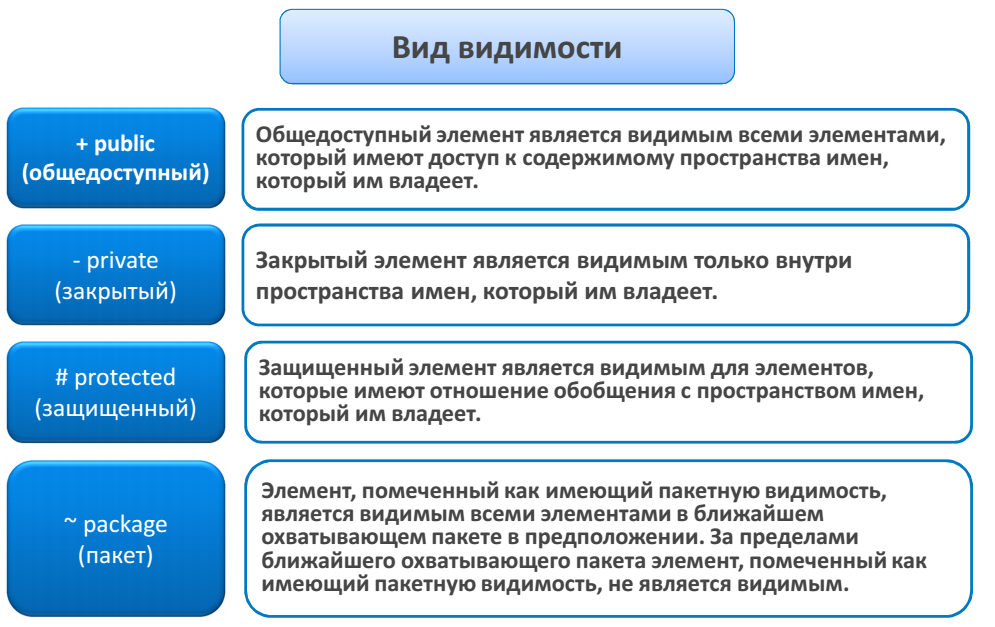
\includegraphics[scale=0.45]{images/lec03-pic22.png}
\end{figure}
\end{frame}

\begin{frame}[t]{Диаграмма классов}
\begin{figure}[h]
\centering
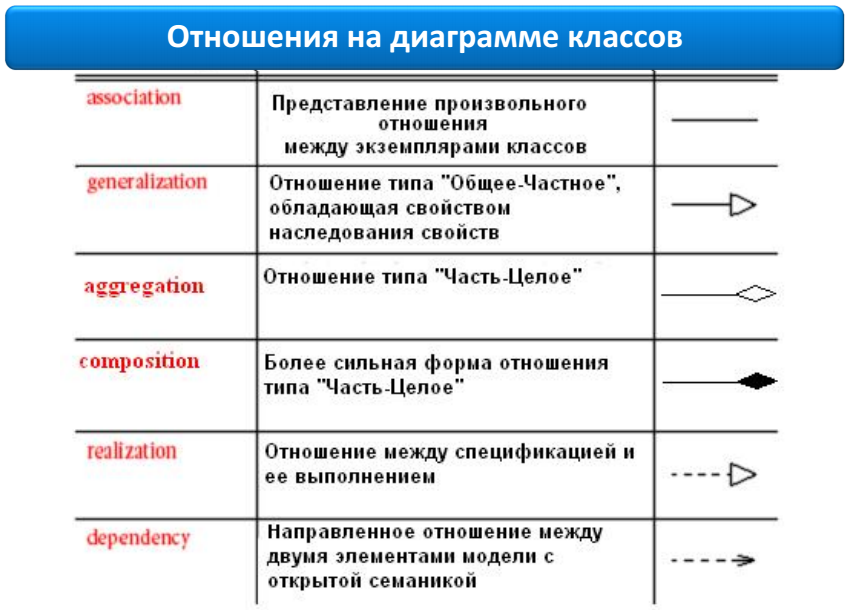
\includegraphics[scale=0.45]{images/lec03-pic23.png}
\end{figure}
\end{frame}

\begin{frame}[t]{Диаграмма классов}
\begin{figure}[h]
\centering
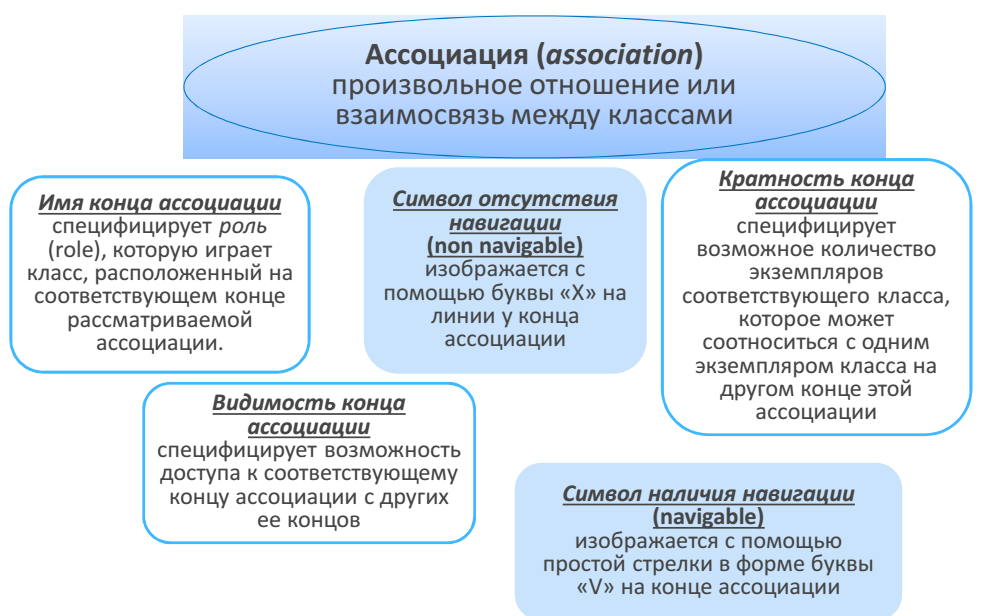
\includegraphics[scale=0.45]{images/lec03-pic24.png}
\end{figure}
\end{frame}

\begin{frame}[t]{Диаграмма классов}
\begin{figure}[h]
\centering
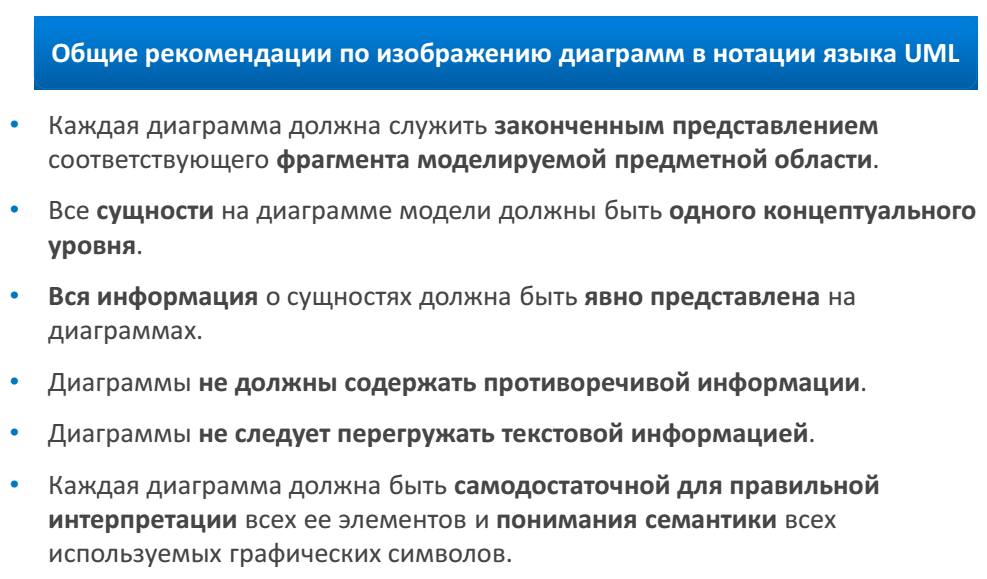
\includegraphics[scale=0.45]{images/lec03-pic25.png}
\end{figure}
\end{frame}

\subsection{Прочие диаграммыю, пример}

\begin{frame}[t]{Диаграмма классов}
\begin{figure}[h]
\centering
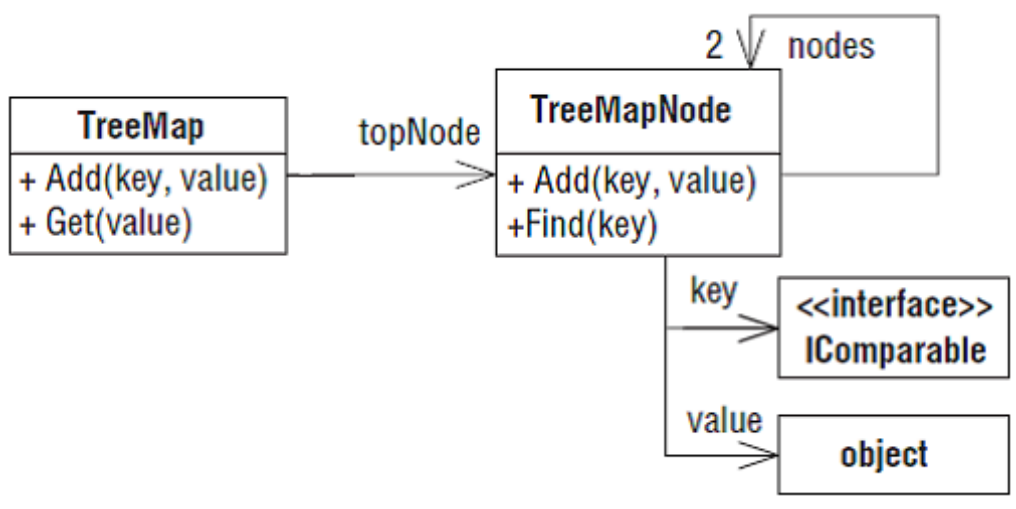
\includegraphics[scale=0.45]{images/lec03-pic26.png}
\end{figure}
\end{frame}

\begin{frame}[t]{Диаграмма объектов}
\begin{figure}[h]
\centering
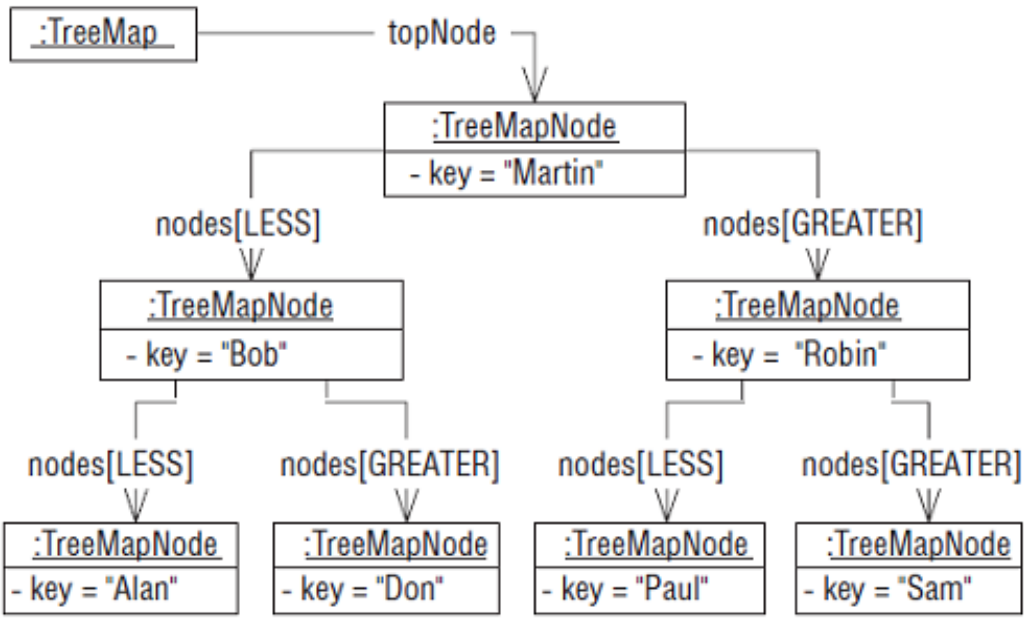
\includegraphics[scale=0.4]{images/lec03-pic27.png}
\end{figure}
\end{frame}

\begin{frame}[t]{Диаграмма последовательности}
\begin{figure}[h]
\centering
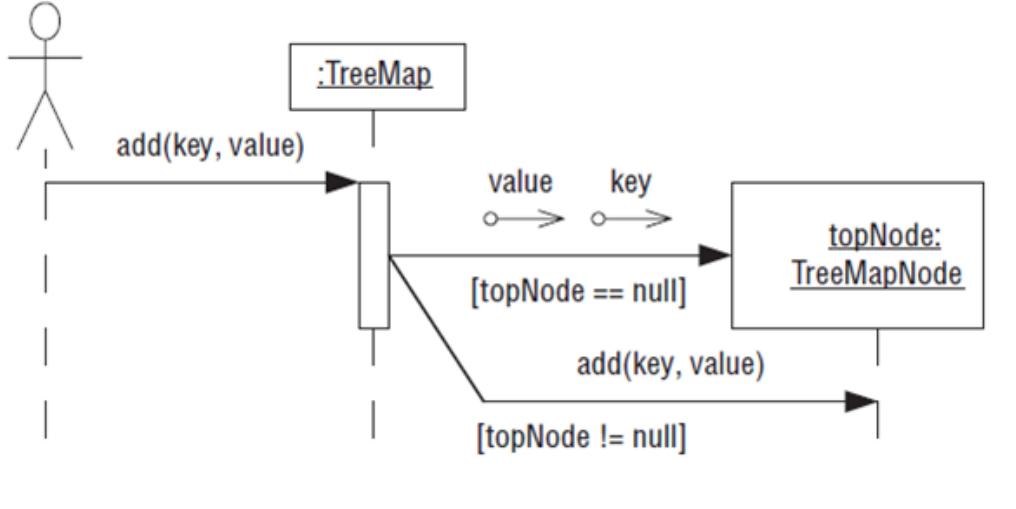
\includegraphics[scale=0.45]{images/lec03-pic28.png}
\end{figure}
\end{frame}

\begin{frame}[t]{Диаграмма взаимодействия}
\begin{figure}[h]
\centering
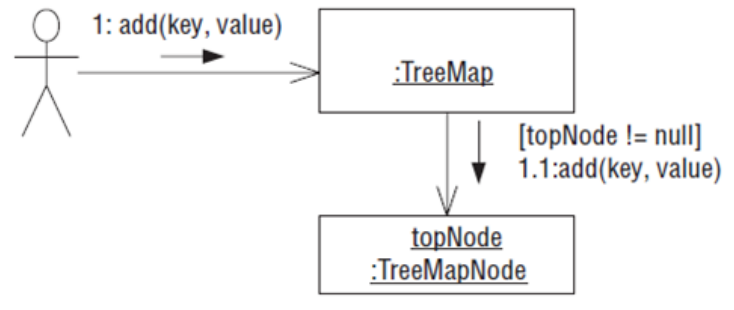
\includegraphics[scale=0.45]{images/lec03-pic29.png}
\end{figure}
\end{frame}

\begin{frame}[t]{Диаграмма состояний}
\begin{figure}[h]
\centering
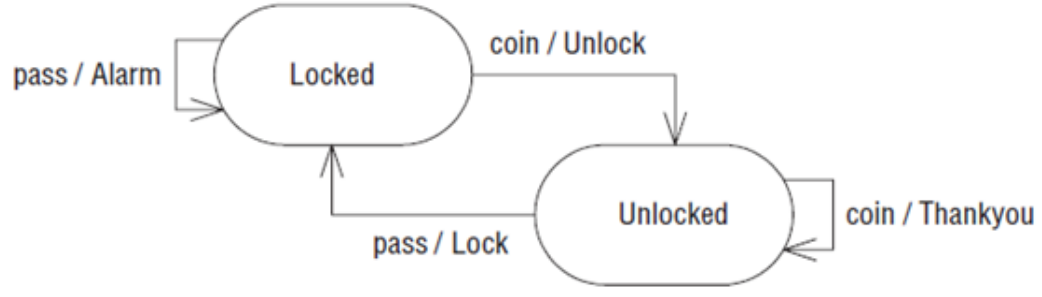
\includegraphics[scale=0.45]{images/lec03-pic30.png}
\end{figure}
\end{frame}

\end{document}
